\section{OPQ View}
\label{sec:opq-view}

The final component of the OPQ Sensor Network system architecture is called OPQ View. It is a web application, implemented using the Meteor application framework, which provides a variety of visualization and query services.  An example of the OPQ View home page is provided in Figure \ref{fig:opq-view-home}.

\begin{figure}
\center 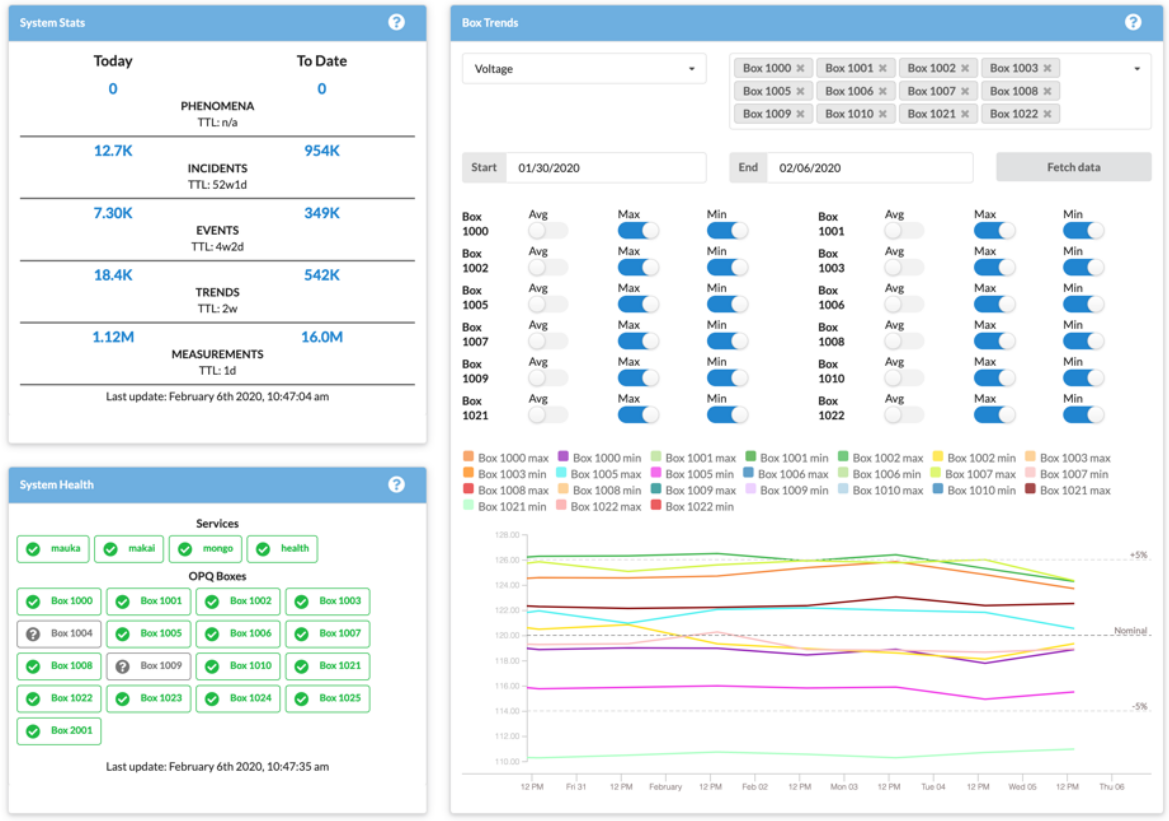
\includegraphics[width=5in]{images/view/homepage.png}
\caption{OPQ View: home page}
\label{fig:opq-view-home}
\end{figure}

The home page provides three components:  a "System Stats" window which indicates the number of data elements currently at each level of the OPQ Mauka data hierarchy, a "System Health" window that indicates whether or not the Cloud services appear to be running correctly and the status of communication with all known OPQ Boxes on the sensor network, and a "Box Trends" visualization that provides the ability to quickly see trends in the four basic measures (Voltage, Frequency, THD, and Transients) over time.

{\em Anthony: a couple of questions about this home page image. First, no phenomena? What's up with that? Second, although the TTL for Measurements is set to 1 day, the System Status window says there are 16M measurements. It seems to me that with 1 measurement per second per box, we should only have around 1.2M per day, so at most double that given the TTL.  Can you explain to me what's happening? }

Figure \ref{fig:opq-view-box-map} shows a map-based view of the sensor network. This figure shows the location of 11 OPQ Boxes on the University of Hawaii campus at one point during Fall of 2019. Depending on the zoom level of the interface, some boxes are collapsed into disks with a number indicating the number of boxes at that location. Zooming in reveals more information about the box including near-real time values for voltage and frequency, as is shown for the box in the upper right corner of the figure.

\begin{figure}
\center 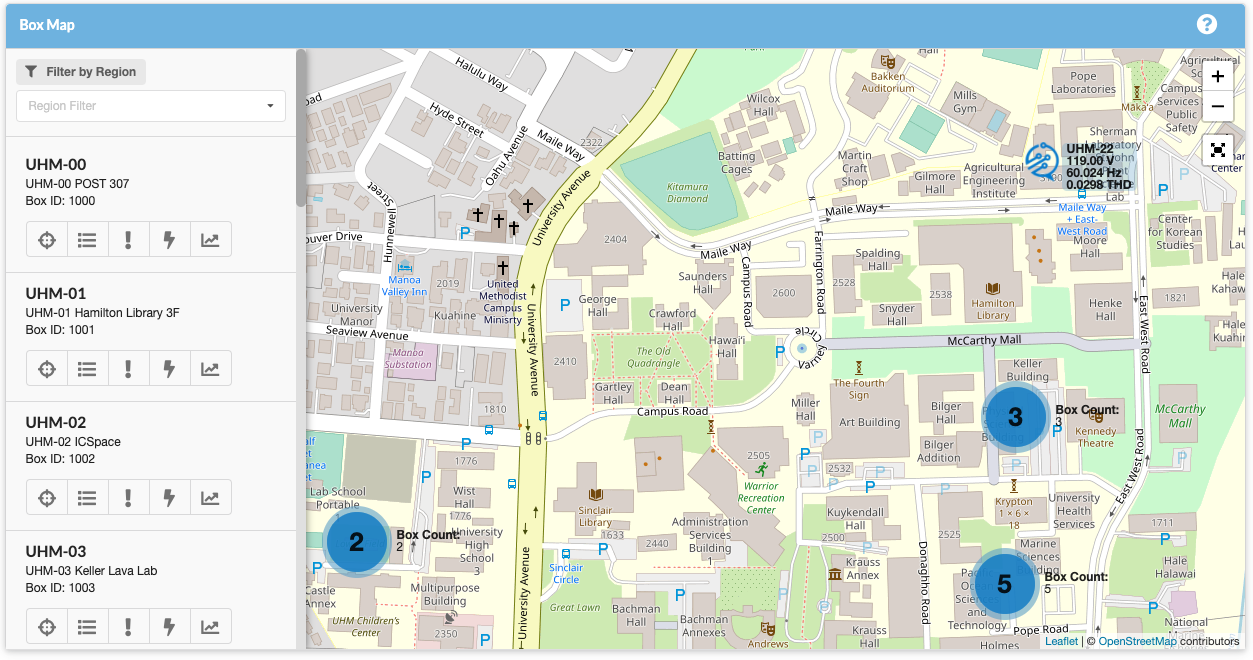
\includegraphics[width=5in]{images/view/boxmap-2.png}
\caption{OPQ View: Box Map}
\label{fig:opq-view-box-map}
\end{figure}

Figure \ref{fig:opq-view-incident-summary} shows a visual display of a single Incident. This view includes a map-based location of the box whose data was involved in the Incident, the start and end time and duration of the Incident, the classification(s) of the anomalous data, and the waveform associated with the Incident (when applicable).

\begin{figure}
\center 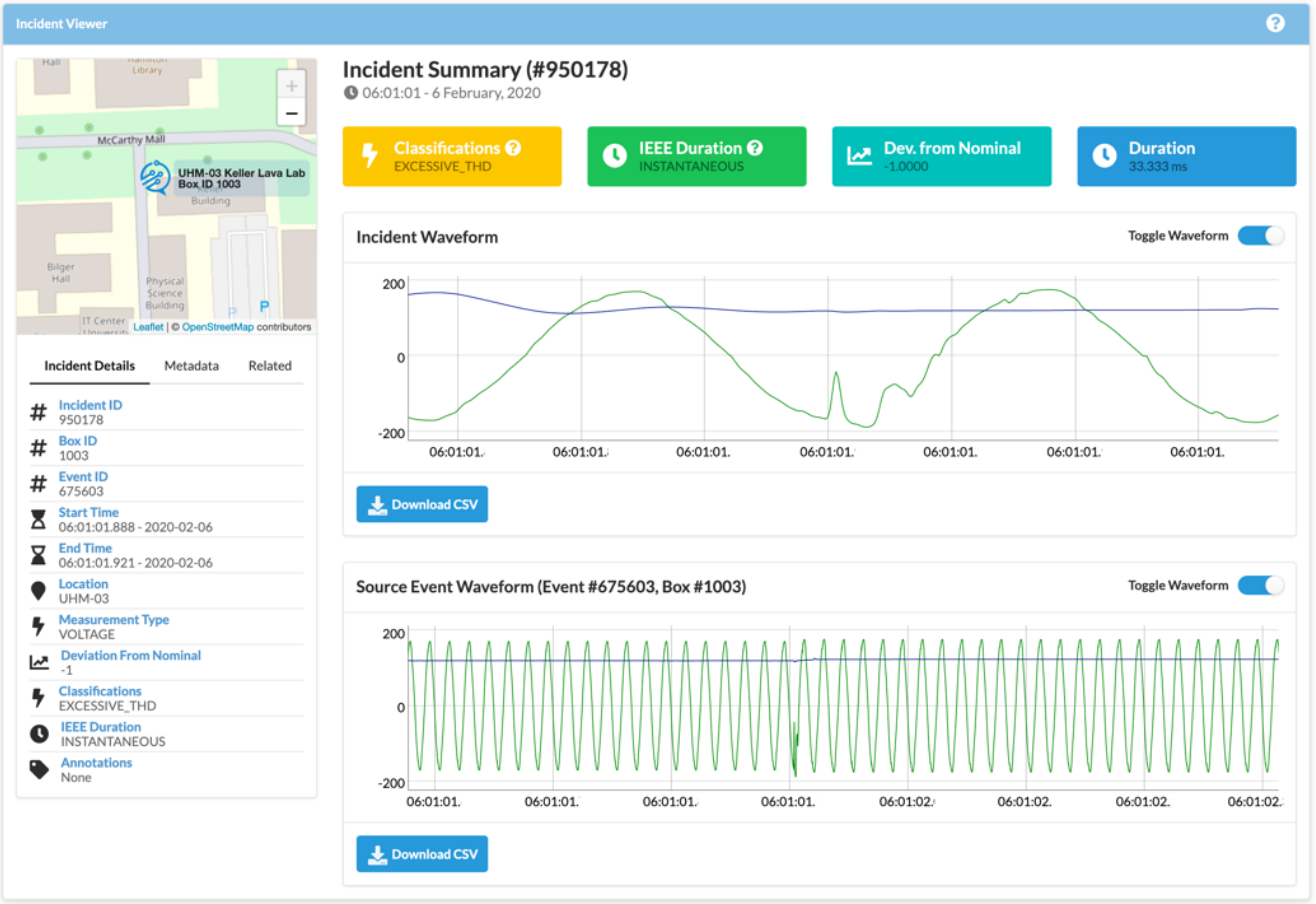
\includegraphics[width=5in]{images/view/incident-summary.png}
\caption{OPQ View: Incident Summary}
\label{fig:opq-view-incident-summary}
\end{figure}

The above images provide a sense for how OPQ View helps users to understand, monitor, and assess an OPQ Sensor Network and the underlying power quality of the grid it is attached to. There are several features in OPQ View for user and box management; for details, please see the OPQ View documentation.


